\documentclass[aspectratio=1610]{beamer}
\usetheme{boxes}
\usecolortheme{crane}
\usepackage{amsmath,amsfonts}
\usepackage{algpseudocode}
\usepackage{multicol}
\usepackage{pgfplots}
\pgfplotsset{compat=1.15}
\usepackage{mathrsfs}
\usetikzlibrary{arrows}


%-------------------------------------------------------------------
%	 TITLE SLIDE
%-------------------------------------------------------------------


\begin{document}

% -------------------------------------------------------------------
% Lesson 2
% -------------------------------------------------------------------
\section{Software specifications. Formal methods}

\begin{frame}
\begin{center}
\Huge Lesson 2\\~\\
\textbf{Software specifications. Formal methods}
\end{center}
\end{frame}


\begin{frame}
\frametitle{Lesson 2}

\Huge In this lesson we will talk about:
 \alert{Software specifications},
 \alert{Formal software specifications, Formal methods},
 \alert{Software verification and validation}
\end{frame}



\begin{frame}
\begin{center}
\Huge
\begin{quote}
\textbf{"Todays software has grown by evolution, not by intelligent design"}
\begin{flushright}
{--- Leslie Lamport}	
\end{flushright}
\end{quote}
\end{center}
\end{frame}


\begin{frame}{Lesson 2}{}
\includegraphics[scale=0.30]{Images/loc.png}
\end{frame}


\begin{frame}{Lesson 2}{}
\begin{center}
\Huge\textbf{Software Specifications}
\end{center}
\end{frame}


\begin{frame}{Lesson 2}{}
\Huge{What is a computer specification?}
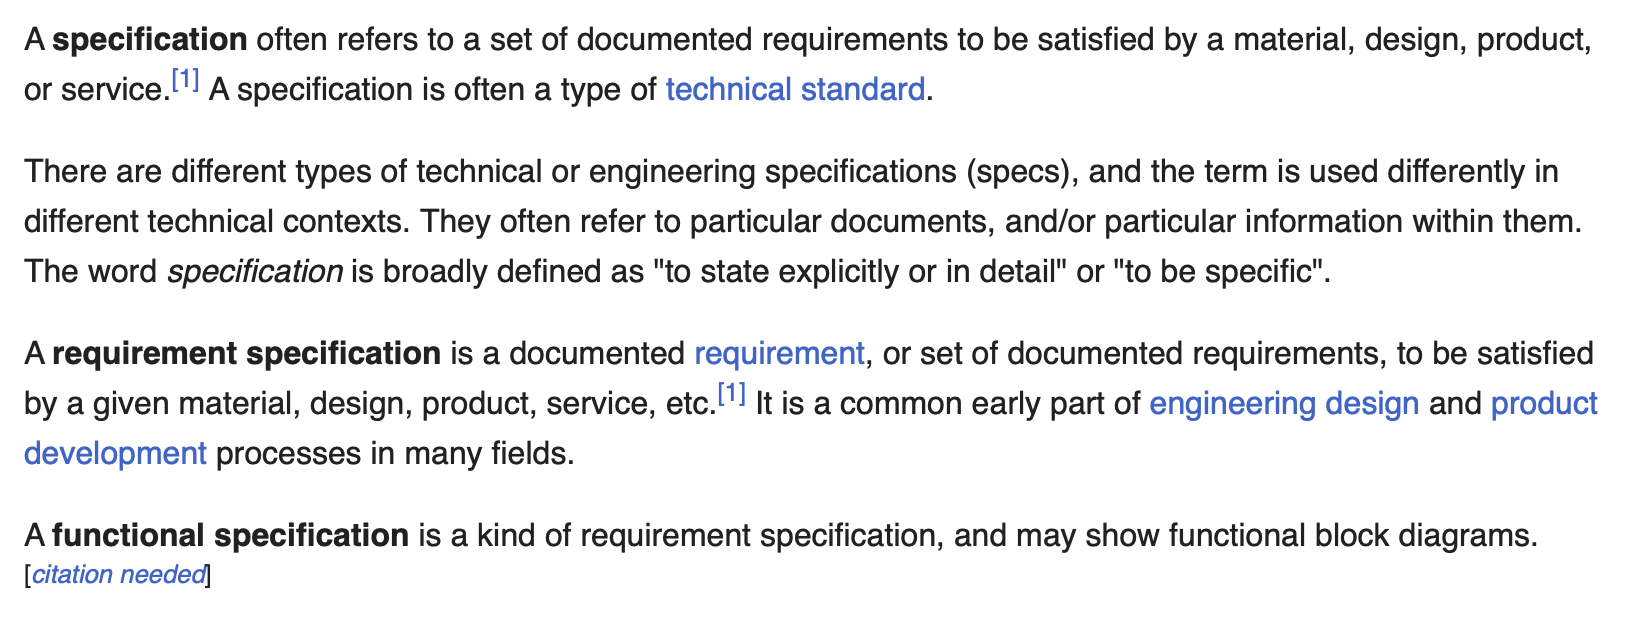
\includegraphics[scale=0.52]{Images/specs}
\end{frame}






\end{document}

